% -----------------------------*- LaTeX -*------------------------------
\documentclass[UTF8]{report}
% ------------------------------------------------------------------------
% Packages
% ------------------------------------------------------------------------
\usepackage{adjustbox}
\usepackage{algorithm,algorithmicx}
\usepackage[noend]{algpseudocode}
\usepackage{amsmath,amsfonts,amssymb,bm,amsthm}%数学宏包、数学字体、数学符号、支持 \mathscr{} 字体、支持粗斜体 \bm{}、数学定理
\usepackage{bigstrut,multirow,rotating}%Excel表格自动导入latex
\usepackage{booktabs}
\usepackage{breqn}
\usepackage{caption}
\usepackage{color}%支持颜色改变
\usepackage{ctex}
\usepackage{enumitem}%自定义列表环境
\usepackage{esint}%支持多种积分算子
\usepackage{extarrows}%任意长度的箭头
\usepackage{fancyhdr}
\usepackage{fontsize}
\usepackage{fontspec}
\usepackage[body={7in, 9in},left=1in,right=1in]{geometry}
\usepackage{graphicx}%支持 \includegraphics{} 插图
\usepackage{mathrsfs}
\usepackage{mathtools}%数学宏包的重要补充
\usepackage[framemethod=TikZ]{mdframed}
\usepackage{nicefrac}
\usepackage{scribe}
\usepackage{subfigure}%插入子图
\usepackage{tikz,xcolor}%画图、画 Feynman 图
\usepackage{upgreek}%数学环境的直立希腊字母
% ------------------------------------------------------------------------
% Macros
% ------------------------------------------------------------------------
%~~~~~~~~~~~~~~~
% Utility latin
%~~~~~~~~~~~~~~~
\newcommand{\ie}{\textit{i.e.}}
\newcommand{\eg}{\textit{e.g.}}
%~~~~~~~~~~~~~~~
% Environment shortcuts
%~~~~~~~~~~~~~~~
\newcommand{\balign}[1]{\ealign{\begin{align}#1\end{align}}}
\newcommand{\baligns}[1]{\ealigns{\begin{align*}#1\end{align*}}}
\newcommand{\bitemize}[1]{\eitemize{\begin{itemize}#1\end{itemize}}}
\newcommand{\benumerate}[1]{\eenumerate{\begin{enumerate}#1\end{enumerate}}}
%~~~~~~~~~~~~~~~
% Text with quads around it
%~~~~~~~~~~~~~~~
\newcommand{\qtext}[1]{\quad\text{#1}\quad}
%~~~~~~~~~~~~~~~
% Shorthand for math formatting
%~~~~~~~~~~~~~~~
\newcommand{\mbb}[1]{\mathbb{#1}}
\newcommand{\mbi}[1]{\boldsymbol{#1}} % Bold and italic (math bold italic)
\newcommand{\mbf}[1]{\mathbf{#1}}
\newcommand{\mc}[1]{\mathcal{#1}}
\newcommand{\mrm}[1]{\mathrm{#1}}
\newcommand{\tbf}[1]{\textbf{#1}}
\newcommand{\tsc}[1]{\textsc{#1}}
%\def\<{{\langle}}
%\def\>{{\rangle}}
\newcommand{\sT}{\sf T}
\newcommand{\grad}{\nabla}
\newcommand{\Proj}{\Pi}
%~~~~~~~~~~~~~~~
% Common sets 定义数集符号
%~~~~~~~~~~~~~~~
\newcommand{\R}{\mathbb{R}}
\newcommand{\Z}{\mathbb{Z}}
\newcommand{\Q}{\mathbb{Q}}
\newcommand{\N}{\mathbb{N}}
\newcommand{\C}{\mathbb{C}}
\newcommand{\reals}{\mathbb{R}} % Real number symbol
\newcommand{\integers}{\mathbb{Z}} % Integer symbol
\newcommand{\rationals}{\mathbb{Q}} % Rational numbers
\newcommand{\naturals}{\mathbb{N}} % Natural numbers
\newcommand{\complex}{\mathbb{C}} % Complex numbers
%~~~~~~~~~~~~~~~
% Common functions
%~~~~~~~~~~~~~~~
\renewcommand{\exp}[1]{\operatorname{exp}\left(#1\right)} % Exponential
\newcommand{\indic}[1]{\mbb{I}\left(#1\right)} % Indicator function
\newcommand{\indicsub}[2]{\mbb{I}_{#2}\left(#1\right)} % Indicator function
\newcommand{\argmax}{\mathop\mathrm{arg\, max}} % Defining math symbols
\newcommand{\argmin}{\mathop\mathrm{arg\, min}}
\renewcommand{\arccos}{\mathop\mathrm{arccos}}
\newcommand{\dom}{\mathop\mathrm{dom}} % Domain
\newcommand{\range}{\mathop\mathrm{range}} % Range
\newcommand{\diag}{\mathop\mathrm{diag}}
\newcommand{\tr}{\mathop\mathrm{tr}}
\newcommand{\abs}{\mathop\mathrm{abs}}
\newcommand{\card}{\mathop\mathrm{card}}
\newcommand{\sign}{\mathop\mathrm{sign}}
\newcommand{\prox}{\mathrm{prox}} % prox
\newcommand{\rank}[1]{\mathrm{rank}(#1)}
\newcommand{\supp}[1]{\mathrm{supp}(#1)}
\newcommand{\norm}[1]{\lVert#1\rVert}
%~~~~~~~~~~~~~~~
% Common probability symbols
%~~~~~~~~~~~~~~~
\newcommand{\family}{\mathcal{P}} % probability family / statistical model
\newcommand{\iid}{\stackrel{\mathrm{iid}}{\sim}}
\newcommand{\ind}{\stackrel{\mathrm{ind}}{\sim}}
\newcommand{\E}{\mathbb{E}} % Expectation symbol
\newcommand{\Earg}[1]{\E\left[#1\right]}
\newcommand{\Esubarg}[2]{\E_{#1}\left[#2\right]}
\renewcommand{\P}{\mathbb{P}} % Probability symbol
\newcommand{\Parg}[1]{\P\left(#1\right)}
\newcommand{\Psubarg}[2]{\P_{#1}\left[#2\right]}
%\newcommand{\Cov}{\mrm{Cov}} % Covariance symbol
%\newcommand{\Covarg}[1]{\Cov\left[#1\right]}
%\newcommand{\Covsubarg}[2]{\Cov_{#1}\left[#2\right]}
%\newcommand{\model}{\mathcal{P}} % probability family / statistical model
%~~~~~~~~~~~~~~~
% Distributions
%~~~~~~~~~~~~~~~
%\newcommand{\Gsn}{\mathcal{N}}
%\newcommand{\Ber}{\textnormal{Ber}}
%\newcommand{\Bin}{\textnormal{Bin}}
%\newcommand{\Unif}{\textnormal{Unif}}
%\newcommand{\Mult}{\textnormal{Mult}}
%\newcommand{\NegMult}{\textnormal{NegMult}}
%\newcommand{\Dir}{\textnormal{Dir}}
%\newcommand{\Bet}{\textnormal{Beta}}
%\newcommand{\Gam}{\textnormal{Gamma}}
%\newcommand{\Poi}{\textnormal{Poi}}
%\newcommand{\HypGeo}{\textnormal{HypGeo}}
%\newcommand{\GEM}{\textnormal{GEM}}
%\newcommand{\BP}{\textnormal{BP}}
%\newcommand{\DP}{\textnormal{DP}}
%\newcommand{\BeP}{\textnormal{BeP}}
%\newcommand{\Exp}{\textnormal{Exp}}
%~~~~~~~~~~~~~~~
% Theorem-like environments
%~~~~~~~~~~~~~~~
%\theoremstyle{definition}
%\newtheorem{definition}{Definition}
%\newtheorem{example}{Example}
%\newtheorem{problem}{Problem}
%\newtheorem{lemma}{Lemma}
%~~~~~~~~~~~~~~~
% 组合数学的模板和作业里用到的一些宏包和自定义命令
%~~~~~~~~~~~~~~~
\renewcommand{\emph}[1]{\begin{kaishu}#1\end{kaishu}}
\newcommand{\falfac}[1]{^{\underline{#1}}}
\newcommand{\binomfrac}[2]{\frac{#1^{\underline{#2}}}{#2!}}
\newcommand{\ceil}[1]{\left\lceil #1 \right\rceil}
\newcommand{\floor}[1]{\left\lfloor #1 \right\rfloor}
\newcommand{\suminfty}[2]{\sum_{#1=#2}^{\infty}}
\newcommand{\suminftyk}[0]{\sum_{k=0}^{\infty}}
\newcommand{\sumint}[3]{\sum_{#1=#2}^{#3}}
\newcommand{\sumintk}[2]{\sum_{k=#1}^{#2}}
\newcommand{\suminti}[2]{\sum_{i=#1}^{#2}}
%~~~~~~~~~~~~~~~
% 定义新命令
%~~~~~~~~~~~~~~~
\newcommand*{\unit}[1]{\mathop{}\!\mathrm{#1}}
\newcommand*{\dif}{\mathop{}\!\mathrm{d}}%微分算子 d
\newcommand*{\pdif}{\mathop{}\!\partial}%偏微分算子
\newcommand*{\cdif}{\mathop{}\!\nabla}%协变导数、nabla 算子
\newcommand*{\laplace}{\mathop{}\!\Delta}%laplace 算子
\newcommand*{\deriv}[2]{\frac{\mathrm{d} #1}{\mathrm{d} {#2}}}
\newcommand*{\derivh}[3]{\frac{\mathrm{d}^{#1} #2}{\mathrm{d} {#3^{#1}}}}
\newcommand*{\pderiv}[2]{\frac{\partial #1}{\partial {#2}}}
\newcommand*{\pderivh}[3]{\frac{\partial^{#1} #2}{\partial {#3^{#1}}}}
\newcommand*{\dderiv}[2]{\dfrac{\mathrm{d} #1}{\mathrm{d} {#2}}}
\newcommand*{\dderivh}[3]{\dfrac{\mathrm{d}^{#1} #2}{\mathrm{d} {#3^{#1}}}}
\newcommand*{\dpderiv}[2]{\dfrac{\partial #1}{\partial {#2}}}
\newcommand*{\dpderivh}[3]{\dfrac{\partial^{#1} #2}{\partial {#3^{#1}}}}
\newcommand{\me}[1]{\mathrm{e}^{#1}}%e 指数
\newcommand{\mi}{\mathrm{i}}%虚数单位
%\newcommand{\mc}{\mathrm{c}}%光速 定义与mathcal冲突
\newcommand{\red}[1]{\textcolor{red}{#1}}
\newcommand{\blue}[1]{\textcolor{blue}{#1}}
%\newcommand{\Rome}[1]{\setcounter{rome}{#1}\Roman{rome}}
%~~~~~~~~~~~~~~~
% 公式环境中箭头符号的简写
%~~~~~~~~~~~~~~~
\newcommand{\ra}{\rightarrow}
\newcommand{\Ra}{\Rightarrow}
\newcommand{\la}{\leftarrow}
\newcommand{\La}{\Leftarrow}
\newcommand{\lra}{\leftrightarrow}
\newcommand{\Lra}{\Leftrightarrow}
\newcommand{\lgla}{\longleftarrow}
\newcommand{\Lgla}{\Longleftarrow}
\newcommand{\lgra}{\longrightarrow}
\newcommand{\Lgra}{\Longrightarrow}
\newcommand{\lglra}{\longleftrightarrow}
\newcommand{\Lglra}{\Longleftrightarrow}
%~~~~~~~~~~~~~~~
% 本.tex文档中特殊定义命令
%~~~~~~~~~~~~~~~
\newcommand{\cdclass}[2]{[#1]_{\text{#2}}}
\newcommand{\spz}{\phantom{0}}
%~~~~~~~~~~~~~~~
% 一些数学的环境设置
%~~~~~~~~~~~~~~~
%\newcounter{counter_exm}\setcounter{counter_exm}{1}
%\newcounter{counter_prb}\setcounter{counter_prb}{1}
%\newcounter{counter_thm}\setcounter{counter_thm}{1}
%\newcounter{counter_lma}\setcounter{counter_lma}{1}
%\newcounter{counter_dft}\setcounter{counter_dft}{1}
%\newcounter{counter_clm}\setcounter{counter_clm}{1}
%\newcounter{counter_cly}\setcounter{counter_cly}{1}
%\newtheorem{theorem}{{\hskip 1.7em \bf 定理}}
%\newtheorem{lemma}[theorem]{\hskip 1.7em 引理}
%\newtheorem{proposition}[theorem]{Proposition}
%\newtheorem{claim}[theorem]{\hskip 1.7em 命题}
%\newtheorem{corollary}[theorem]{\hskip 1.7em 推论}
%\newtheorem{definition}[theorem]{\hskip 1.7em 定义}
\newcommand{\problem}[1]{{\setlength{\parskip}{10pt}\noindent \bf{#1}}}
\newenvironment{solution}{{\noindent\hskip 2em \bf 解 \quad}}{}
\renewenvironment{proof}{{\setlength{\parskip}{7pt}\noindent\hskip 2em \bf 证明 \quad}}{\hfill$\qed$\par}
%\newenvironment{example}{{\noindent\hskip 2em \bf 例 \arabic{counter_exm}\quad}}{\addtocounter{counter_exm}{1}\par}
%\newenvironment{concept}[1]{{\bf #1\quad} \begin{kaishu}} {\end{kaishu}\par}

% ----------------------------------------------------------------------
% Header information
% ------------------------------------------------------------------------

\begin{document}

\course{B0911006Y-01} 			%optional
\coursetitle{Computer Organization and Design}	%optional
\semester{2023 Spring}		%optional
\lecturer{Ke Zhang}	%optional
\scribe{吉骏雄}		%required
\lecturenumber{5}			%required (must be a number)
\lecturedate{April 3}	%required (omit year)

\maketitle

% ----------------------------------------------------------------------
% Body of the document
% ------------------------------------------------------------------------


\textbf{习题:6.20(原码一位乘、原码两位乘、补码一位乘Booth算法必做, 补码两位乘选做), 6.23, 6.21(原码加减交替除法,补码加减交替除法)}

\problem{6.20} 用原码一位乘、两位乘和补码一位乘 (Booth算法) 、两位乘计算$x·y$.

\begin{enumerate}
    \item $x=  0.110 111$ ,  $y= -0.101 110$ ;
    
    \item $x= -0.010 111$ ,  $y= -0.010 101$ ;
    
    \item $x=  19$        ,  $y=  35$        ;
    
    \item $x=  0.110 11$  ,  $y= -0.111 01$  .
\end{enumerate}

\begin{solution}
    \begin{enumerate}
        \item $x=  0.110 111$ ,  $y= -0.101 110$ ;
        
        原码一位乘:
        \begin{tabular}{cc|c|c}
             & 部分积     & 乘数     & \\
            \hline
             & 0.000000 & 101110  &         \\
            +& 0.000000 &         & $+0$    \\
            \hline
             & 0.000000 &         &         \\
             & 0.000000 & 0 10111 & $\ra 1$ \\
            +& 0.110111 &  & $+x$    \\
            \hline
             & 0.110111 &  &         \\
             & 0.011011 & 10 1011 & $\ra 1$ \\
            +& 0.110111 &  & $+x$    \\
            \hline
             & 1.010010 &  &         \\
             & 0.101001 & 010 101 & $\ra 1$ \\
            +& 0.110111 &  & $+x$    \\
            \hline
             & 1.100000 &  &         \\
             & 0.110000 & 0010 10 & $\ra 1$ \\
            +& 0.000000 &  & $+0$    \\
            \hline
             & 0.110000 &  &         \\
             & 0.011000 & 00010 1 & $\ra 1$ \\
            +& 0.110111 &  & $+x$    \\
            \hline
             & 1.001111 &  &         \\
             & 0.100111 & 100010  & $\ra 1$ \\
        \end{tabular}

        符号位异或为1, 结果的原码为: 1.100111 100010
        
        原码两位乘:
        \begin{tabular}{cc|l|c|c}
             & 部分积      & 乘数      & $C_j$ & \\
            \hline
             & 000.000000 & 00.101110 & 0 & \\
            +& 001.101110 &           &   & $+2x$ \\
            \hline
             & 001.101110 &           &   & \\
             & 000.011011 & 10 001011 & 0 & $\ra 2$ \\
            +& 111.001001 &           &   & $-x $ \\
            \hline
             & 111.100100 &           &   & \\
             & 111.111001 & 0010 0010 & 1 & $\ra 2$ \\
            +& 111.001001 &           &   & $-x $ \\
            \hline
             & 111.000010 &           &   & \\
             & 111.110000 & 100010 00 & 1 & $\ra 2$ \\
            +& 000.110111 &           &   & $+x $ \\
            \hline
             & 000.100111 & 100010    &   & \\
        \end{tabular}

        符号位异或为1, 结果的原码为: 1.100111 100010
        
        $\cdclass{x}{补}=  0.110 111$ ,  $\cdclass{y}{补}= 1.010 010$ ;

        Booth算法:
        \begin{tabular}{cc|r|c|c}
             & 部分积      & 乘数      & 附加位 & \\
            \hline
             & 00.000000 & 1.010010  & 0 & $+0,\ \ra 1$ \\
             & 00.000000 & 0 101001 & 0 & $-x$ \\
            +& 11.001001 &          &   &  \\
            \hline
             & 11.001001 &          &   & $\ra 1$ \\
             & 11.100100 & 10 10100 & 1 & $+x$ \\
            +& 00.110111 &          &   &  \\
            \hline
             & 00.011011 &          &   & $\ra 1$ \\
             & 00.001101 & 110 1010 & 0 & $+0,\ \ra 1$ \\
             & 00.000110 & 1110 101 & 0 & $-x$ \\
            +& 11.001001 &          &   &  \\
            \hline
             & 11.001111 &          &   & $\ra 1$ \\
             & 11.100111 & 11110 10 & 1 & $+x$ \\
            +& 00.110111 &          &   &  \\
            \hline
             & 00.011110 &          &   & $\ra 1$ \\
             & 00.001111 & 011110 1 & 0 & $-x$ \\
            +& 11.001001 &          &   &  \\
            \hline
             & 11.011000 & 011110 x &   & \\
        \end{tabular}

        结果的补码为: 1.011000 011110

        \item $x= -0.010 111$ ,  $y= -0.010 101$ ;
        
        原码一位乘:
        \begin{tabular}{cc|l|c}
             & 部分积     & 乘数     & \\
            \hline
             & 0.000000 & 010101  &         \\
            +& 0.010111 &         & $+x$    \\
            \hline
             & 0.010111 &         &         \\
             & 0.001011 & 1 01010 & $\ra 1$ \\
            +& 0.000000 &         & $+0$    \\
            \hline
             & 0.001011 &         &         \\
             & 0.000101 & 11 0101 & $\ra 1$ \\
            +& 0.010111 &         & $+x$    \\
            \hline
             & 0.011100 &         &         \\
             & 0.001110 & 011 010 & $\ra 1$ \\
            +& 0.000000 &         & $+0$    \\
            \hline
             & 0.001110 &         &         \\
             & 0.000111 & 0011 01 & $\ra 1$ \\
            +& 0.010111 &         & $+x$    \\
            \hline
             & 0.011110 &         &         \\
             & 0.001111 & 00011 0 & $\ra 1$ \\
            +& 0.000000 &         & $+0$    \\
            \hline
             & 0.001111 &         &         \\
             & 0.000111 & 100011  & $\ra 1$ \\
        \end{tabular}
        
        符号位异或为0, 结果的原码为: 0.000111 100011
        
        原码两位乘:
        \begin{tabular}{cc|l|c|c}
             & 部分积      & 乘数      & $C_j$ & \\
            \hline
             & 000.000000 & 00.010101 & 0 & \\
            +& 000.010111 &           &   & $+x $ \\
            \hline
             & 000.010111 &           &   & \\
             & 000.000101 & 11 000101 & 0 & $\ra 2$ \\
            +& 000.010111 &           &   & $+x $ \\
            \hline
             & 000.011100 &           &   & \\
             & 000.000111 & 0011 0001 & 0 & $\ra 2$ \\
            +& 000.010111 &           &   & $+x $ \\
            \hline
             & 000.011110 &           &   & \\
             & 000.000111 & 100011 00 & 0 & $\ra 2$ \\
            +& 000.000000 &           &   & $+0 $ \\
            \hline
             & 000.000111 & 100011    &   & \\
        \end{tabular}

        符号位异或为0, 结果的原码为: 0.000111 100011
        
        $\cdclass{x}{补}=  1.101 001$ ,  $\cdclass{y}{补}= 1.101 011$ ;

        Booth算法:
        \begin{tabular}{cc|l|c|c}
             & 部分积      & 乘数      & 附加位 & \\
            \hline
             & 00.000000 & 1.101011 & 0 & $-x$ \\
            +& 00.010111 &          &   &  \\
              \hline
             & 00.010111 &          &   & $\ra 1$ \\
             & 00.001011 & 1 110101 & 1 & $+0,\ \ra 1$ \\
             & 00.000101 & 11 11010 & 1 & $+x$ \\
            +& 11.101001 &          &   &  \\
              \hline
             & 11.101110 &          &   & $\ra 1$ \\
             & 11.110111 & 011 1101 & 0 & $-x$ \\
            +& 00.010111 &          &   &  \\
              \hline
             & 00.001110 &          &   & $\ra 1$ \\
             & 00.000111 & 0011 110 & 1 & $+x$ \\
            +& 11.101001 &          &   &  \\
              \hline
             & 11.110000 &          &   & $\ra 1$ \\
             & 11.111000 & 00011 11 & 0 & $-x$ \\
            +& 00.010111 &          &   &  \\
              \hline
             & 00.001111 &          &   & $\ra 1$ \\
             & 00.000111 & 100011 1 & 1 & $+0$ \\
             & 00.000111 & 100011   &  & \\
        \end{tabular}

        结果的补码为: 0.000111 100011
        
        \item $x=  19 = 0,010 011$        ,  $y=  35 = 0,100 011$        ;
        
        原码一位乘:
        \begin{tabular}{cc|c|c}
             & 部分积     & 乘数     & \\
            \hline
             & 0,000000 & 100011  &         \\
            +& 0,010011 &         & $+x$    \\
            \hline
             & 0,010011 &         &         \\
             & 0,001001 & 1 10001 & $\ra 1$ \\
            +& 0,010011 &         & $+x$    \\
            \hline
             & 0,011100 &         &         \\
             & 0.001110 & 01 1000 & $\ra 1$ \\
            +& 0,000000 &         & $+0$    \\
            \hline
             & 0,001110 &         &         \\
             & 0,000111 & 001 100 & $\ra 1$ \\
            +& 0,000000 &         & $+0$    \\
            \hline
             & 0,000111 &         &         \\
             & 0,000011 & 1001 10 & $\ra 1$ \\
            +& 0,000000 &         & $+0$    \\
            \hline
             & 0,000011 &         &         \\
             & 0,000001 & 11001 1 & $\ra 1$ \\
            +& 0,010011 &         & $+x$    \\
            \hline
             & 0,010100 &         &         \\
             & 0,001010 & 011001 & $\ra 1$ \\
        \end{tabular}
        
        符号位异或为0, 结果的原码为: 0,001010 011001
        
        原码两位乘:
        \begin{tabular}{cc|l|c|c}
             & 部分积      & 乘数      & $C_j$ & \\
            \hline
             & 000.000000 & 00.100011 & 0 & \\
            +& 111.101101 &           &   & $-x $ \\
            \hline
             & 111.101101 &           &   & \\
             & 111.111011 & 01 001000 & 1 & $\ra 2$ \\
            +& 000.010011 &           &   & $+x $ \\
            \hline
             & 000.001110 &           &   & \\
             & 000.000011 & 1001 0010 & 0 & $\ra 2$ \\
            +& 000.100110 &           &   & $+2x $ \\
            \hline
             & 000.101001 &           &   & \\
             & 000.001010 & 011001 00 & 0 & $\ra 2$ \\
            +& 000.000000 &           &   & $+0 $ \\
            \hline
             & 000.001010 & 011001    &   & \\
        \end{tabular}

        符号位异或为0, 结果的原码为: 0,001010 011001
        
        $\cdclass{x}{补}=  0,010011$ ,  $\cdclass{y}{补}= 0,100011$ ;

        Booth算法:
        \begin{tabular}{cc|l|c|c}
             & 部分积      & 乘数      & 附加位 & \\
            \hline
             & 00.000000 & 0.100011 & 0 & $-x$ \\
            +& 11.101101 &          &   &  \\
              \hline
             & 11.101101 &          &   & $\ra 1$ \\
             & 11,110110 & 1 010001 & 1 & $+0,\ \ra 1$ \\
             & 11,111011 & 01 01000 & 1 & $+x$ \\
            +& 00,010011 &          &   &  \\
              \hline
             & 00,001110 &          &   & $\ra 1$ \\
             & 00,000111 & 001 0100 & 0 & $+0,\ \ra 1$ \\
             & 00,000011 & 1001 010 & 0 & $+0,\ \ra 1$ \\
             & 00,000001 & 11001 01 & 0 & $-x$ \\
            +& 11.101101 &          &   &  \\
              \hline
             & 11,101110 &          &   & $\ra 1$ \\
             & 11,110111 & 011001 0 & 1 & $+x$ \\
            +& 00,010011 &          &   &  \\
              \hline
             & 00,001010 & 011001   &   &  \\
        \end{tabular}
        
        结果的补码为: 0,001010 011001

        \item $x=  0.11011$  ,  $y= -0.11101$  .
        
        原码一位乘:
        \begin{tabular}{cc|l|c}
             & 部分积     & 乘数     & \\
            \hline
             & 0.00000 & 11101   &         \\
            +& 0.11011 &         & $+x$    \\
            \hline
             & 0.11011 &         &         \\
             & 0.01101 & 1 1110  & $\ra 1$ \\
            +& 0.00000 &         & $+0$    \\
            \hline
             & 0.01101 &         &         \\
             & 0.00110 & 11 111 & $\ra 1$ \\
            +& 0.11011 &         & $+x$    \\
            \hline
             & 1.00001 &         &         \\
             & 0.10000 & 111 11  & $\ra 1$ \\
            +& 0.11011 &         & $+x$    \\
            \hline
             & 1.01011 &         &         \\
             & 0.10101 & 1111 1  & $\ra 1$ \\
            +& 0.11011 &         & $+x$    \\
            \hline
             & 1.10000 &         &         \\
             & 0.11000 & 01111   & $\ra 1$ \\
        \end{tabular}
        
        符号位异或为1, 结果的原码为: 1.11000 01111
        
        原码两位乘:
        \begin{tabular}{cc|l|c|c}
             & 部分积      & 乘数      & $C_j$ & \\
            \hline
             & 000.00000 & 0.11101   & 0 & \\
            +& 000.11011 &           &   & $+x $ \\
            \hline
             & 000.11011 &           &   & \\
             & 000.00110 & 11 0111   & 0 & $\ra 2$ \\
            +& 111.00101 &           &   & $-x $ \\
            \hline
             & 111.01011 &           &   & \\
             & 111.11010 & 1111 01   & 1 & $\ra 2$ \\
            +& 001.10110 &           &   & $+2x $ \\
            \hline
             & 001.10000 &           &   & \\
             & 000.11000 & 01111     &  & $\ra 1$ (!) \\
        \end{tabular}

        符号位异或为1, 结果的原码为: 1.11000 01111
        
        $\cdclass{x}{补}=  0.11011$ ,  $\cdclass{y}{补}= 1.00011$ ;

        Booth算法:
        \begin{tabular}{cc|l|c|c}
             & 部分积   & 乘数    & 附加位 & \\
            \hline
             & 00.00000 & 1.00011 & 0 & $-x$ \\
            +& 11.00101 &         &   &  \\
              \hline
             & 11.00101 &         &   & $\ra 1$ \\
             & 11.10010 & 1 10001 & 1 & $+0,\ \ra 1$ \\
             & 11.11001 & 01 1000 & 1 & $+x$ \\
            +& 00.11011 &         &   &  \\
              \hline
             & 00.10100 &         &   & $\ra 1$ \\
             & 00.01010 & 001 100 & 0 & $+0,\ \ra 1$ \\
             & 00.00101 & 0001 10 & 0 & $+0,\ \ra 1$ \\
             & 00.00010 & 10001 1 & 0 & $-x$ \\
            +& 11.00101 &         &   &  \\
              \hline
             & 11.00111 & 10001   &   & \\
        \end{tabular}

        结果的补码为: 1.00111 10001
    \end{enumerate}

\end{solution}


\problem{6.23} 画出实现Booth算法的运算器框图, 要求如下: 
\begin{enumerate}
    \item 寄存器和全加器均用方框表示, 指出寄存器和全加器的位数.
    \item 说明加和移位的次数.
    \item 详细画出最低位全加器的输入电路.
    \item 描述Booth算法重复加和移位的过程.
\end{enumerate}

\begin{solution}
    如图\ref{fig:6_23}
    \begin{figure}[htb]
        \centering
        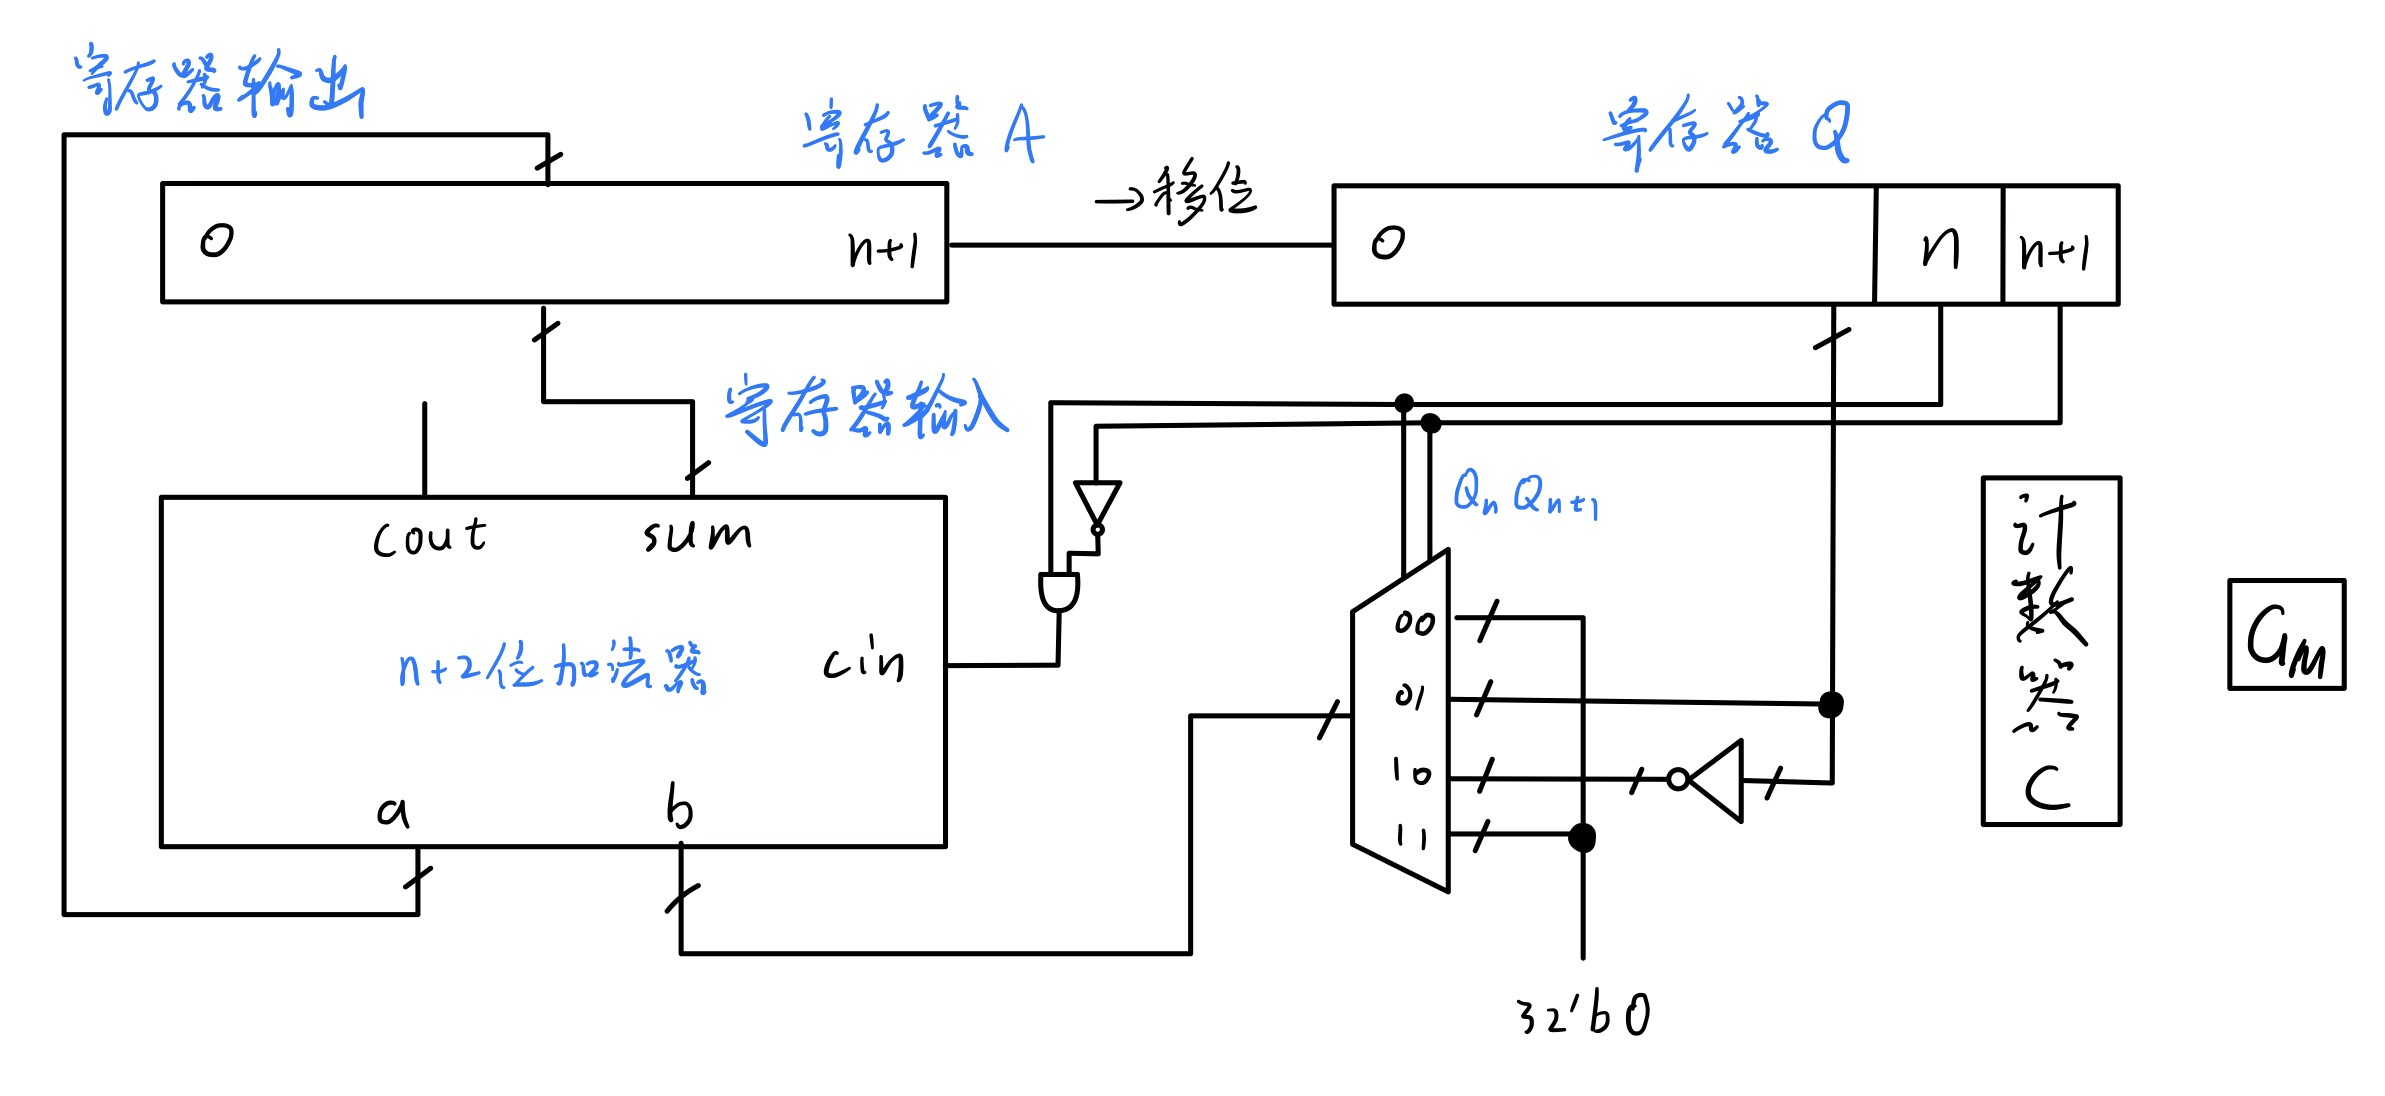
\includegraphics[width=10cm]{fig/6.23.jpg}
        \caption{6.23 Booth算法运算器框图}
        \label{fig:6_23}
    \end{figure}

    寄存器和全加器都是$n+2$位. 加法和移位运算的次数都是$n$次. 

    每个周期 (不一定是单个时钟周期), 取出两个寄存器中的数据, 输入选择器和加法器得到结果, 然后将结果输入回寄存器A. 之后, 将整个寄存器A与Q中的所有数字视为一个整体, 进行算术右移. 这样就结束了一个周期.
\end{solution}


\problem{6.21} 用原码加减交替法和补码加减交替法计算$x\div y$。

\begin{enumerate}
    \item x =  0.100111, y =  0.101011;
    \item x = -0.10101 , y =  0.11011 ;
    \item x =  0.10100 , y = -0.10001 ;
    \item x =  13/32   , y = -27/32   .
\end{enumerate}

\begin{solution}
    \begin{enumerate}
\item x =  0.100111, y =  0.101011;
        
        原码加减交替法:
        \begin{tabular}{cc|r|l}
            & 被除数 (余数)   & 商    & \\
           \hline
            & 0.100111 &  $0.000000 $ &   \\
           +& 1.010101 &         $ $ &  $-y$ \\
           \hline
            & 1.111100 &        $0 $ & 余数为负, 上商为$0$ \\
            & 1.111000 &     $0\spz$ & $\la 1$ \\
           +& 0.101011 &         $ $ &  $+y$ \\
           \hline
            & 0.100011 &       $01 $ & 余数为正, 上商为$1$ \\
            & 1.000110 &    $01\spz$ & $\la 1$ \\
           +& 1.010101 &         $ $ &  $-y$ \\
           \hline
            & 0.011011 &      $011 $ & 余数为正, 上商为$1$ \\
            & 0.110110 &   $011\spz$ & $\la 1$ \\
           +& 1.010101 &         $ $ &  $-y$ \\
           \hline
            & 0.001011 &     $0111 $ & 余数为正, 上商为$1$ \\
            & 0.010110 &  $0111\spz$ & $\la 1$ \\
           +& 1.010101 &         $ $ &  $-y$ \\
           \hline
            & 1.101011 &    $01110 $ & 余数为负, 上商为$0$ \\
            & 1.010110 & $01110\spz$ & $\la 1$ \\
           +& 0.101011 &         $ $ &  $+y$ \\
           \hline
            & 0.000001 &   $011101 $ & 余数为正, 上商为$1$ \\
            & 0.000010 &$011101\spz$ & $\la 1$ \\
           +& 1.010101 &         $ $ & $-y$ \\
           \hline
            & 1.010111 &  $0111010 $ & 余数为负, 上商为$0$ \\
        \end{tabular}

        符号位异或为0, 所以结果为$0.111010$.

        补码加减交替法:
        \begin{tabular}{cc|r|l}
            & 被除数 (余数)   & 商    & \\
           \hline
            & 0.100111 &  $0.000000$ &   \\
           +& 1.010101 &         $ $ & $x,y$符号位同号, $-y$ \\
           \hline
            & 1.111100 &        $0 $ & $R,y$符号位异号, 上商为$0$ \\
            & 1.111000 &     $0\spz$ & $\la 1$ \\
           +& 0.101011 &         $ $ & $+y$ \\
           \hline
            & 0.100011 &       $01 $ & $R,y$符号位同号, 上商为$1$ \\
            & 1.000110 &    $01\spz$ & $\la 1$ \\
           +& 1.010101 &         $ $ & $-y$ \\
           \hline
            & 0.011011 &      $011 $ & $R,y$符号位同号, 上商为$1$ \\
            & 0.110110 &   $011\spz$ & $\la 1$ \\
           +& 1.010101 &         $ $ & $-y$ \\
           \hline
            & 0.001011 &     $0111 $ & $R,y$符号位同号, 上商为$1$ \\
            & 0.010110 &  $0111\spz$ & $\la 1$ \\
           +& 1.010101 &         $ $ & $-y$ \\
           \hline
            & 1.101011 &    $01110 $ & $R,y$符号位异号, 上商为$0$ \\
            & 1.010110 & $01110\spz$ & $\la 1$ \\
           +& 0.101011 &         $ $ & $+y$ \\
           \hline
            & 0.000001 &   $011101 $ & $R,y$符号位同号, 上商为$1$ \\
            & 0.000010 &  $0111011 $ & $\la 1$, 末位置$1$ \\
        \end{tabular}

        答案商的补码为$0.111011$.

\item x = -0.10101 , y =  0.11011 ;
           
        原码加减交替法:
        \begin{tabular}{cc|r|l}
            & 被除数 (余数)   & 商    & \\
           \hline
            & 0.10101  &  $0.00000 $ &   \\
           +& 1.00101  &         $ $ &  $-y$ \\
           \hline
            & 1.11010  &        $0 $ & 余数为负, 上商为$0$ \\
            & 1.10100  &     $0\spz$ & $\la 1$ \\
           +& 0.11011  &         $ $ &  $+y$ \\
           \hline
            & 0.01111  &       $01 $ & 余数为正, 上商为$1$ \\
            & 0.11110  &    $01\spz$ & $\la 1$ \\
           +& 1.00101  &         $ $ &  $-y$ \\
           \hline
            & 0.00011  &      $011 $ & 余数为正, 上商为$1$ \\
            & 0.00110  &   $011\spz$ & $\la 1$ \\
           +& 1.00101  &         $ $ &  $-y$ \\
           \hline
            & 1.01011  &     $0110 $ & 余数为负, 上商为$0$ \\
            & 0.10110  &  $0111\spz$ & $\la 1$ \\
           +& 0.11011  &         $ $ &  $+y$ \\
           \hline
            & 1.10001  &    $01100 $ & 余数为负, 上商为$0$ \\
            & 1.00010  & $01100\spz$ & $\la 1$ \\
           +& 0.11011  &         $ $ &  $+y$ \\
           \hline
            & 1.11101  &   $011000 $ & 余数为负, 上商为$0$ \\
           +& 0.11011  &         $ $ & 恢复余数 $+y$ \\
           \hline
            & 0.11000  &   $011000 $ &  \\
        \end{tabular}

        符号位异或为1, 所以商结果原码为$1.11000$, 补码为$1.01000$, 余数为$0.11000$

        补码加减交替法:
        \begin{tabular}{cc|r|l}
            & 被除数 (余数)   & 商    & \\
           \hline
            & 1.01011 &  $0.00000$ &   \\
           +& 0.11011 &         $ $ & $x,y$符号位异号, $+y$ \\
           \hline
            & 0.00110 &        $1 $ & $R,y$符号位同号, 上商为$1$ \\
            & 0.01100 &     $1\spz$ & $\la 1$ \\
           +& 1.00101 &         $ $ & $-y$ \\
           \hline
            & 1.10001 &       $10 $ & $R,y$符号位异号, 上商为$0$ \\
            & 1.00010 &    $10\spz$ & $\la 1$ \\
           +& 0.11011 &         $ $ & $+y$ \\
           \hline
            & 1.11101 &      $100 $ & $R,y$符号位异号, 上商为$0$ \\
            & 1.11010 &   $100\spz$ & $\la 1$ \\
           +& 0.11011 &         $ $ & $+y$ \\
           \hline
            & 0.10101 &     $1001 $ & $R,y$符号位同号, 上商为$1$ \\
            & 1.01010 &  $1001\spz$ & $\la 1$ \\
           +& 1.00101 &         $ $ & $-y$ \\
           \hline
            & 0.01111 &    $10011 $ & $R,y$符号位同号, 上商为$1$ \\
            & 0.11110 &   $100111 $ & $\la 1$, 末位置$1$ \\
        \end{tabular}

        商的补码为$1.00111$.

\item x =  0.10100 , y = -0.10001 ;

        原码加减交替法:
        \begin{tabular}{cc|r|l}
            & 被除数 (余数)   & 商    & \\
           \hline
            & 0.10100  &  $0.00000 $ &   \\
           +& 1.01111  &         $ $ &  $-y$ \\
           \hline
            & 0.00011  &        $1 $ & 余数为正, 上商为$1$, 产生溢出 \\
        %     & 0.00110  &     $1\spz$ & $\la 1$ \\
        %    +& 1.01111  &         $ $ & $-y$ \\
        %    \hline
        %     & 1.10101  &       $10 $ & 余数为负, 上商为$0$ \\
        %     & 1.01010  &    $10\spz$ & $\la 1$ \\
        %    +& 0.10001  &         $ $ & $+y$ \\
        %    \hline
        %     & 1.11011  &      $100 $ & 余数为负, 上商为$0$ \\
        %     & 1.10110  &  $100\spz$  & $\la 1$ \\
        %    +& 0.10001  &         $ $ & $+y$ \\
        %    \hline
        %     & 0.00111  &     $1001 $ & 余数为正, 上商为$1$ \\
        %     & 0.01110  &  $1001\spz$ & $\la 1$ \\
        %    +& 1.01111  &         $ $ & $-y$ \\
        %    \hline
        %     & 1.11101  &    $10010 $ & 余数为负, 上商为$0$ \\
        %     & 1.11010  & $10010\spz$ & $\la 1$ \\
        %    +& 0.10001  &         $ $ & $+y$ \\
        %    \hline
        %     & 0.01011  &   $100101 $ & 余数为正, 上商为$1$ \\
        \end{tabular}

        % 符号位异或为1, 所以商结果原码为$1.11000$, 补码为$1.01000$, 余数为$0.11000$

        补码加减交替法:
        \begin{tabular}{cc|r|l}
            & 被除数 (余数)   & 商    & \\
           \hline
            & 0.10100 &  $0.00000$ &   \\
           +& 1.01111 &         $ $ & $x,y$符号位异号, $+y$ \\
           \hline
            & 0.00011 &        $0 $ & $R,y$符号位异号, 上商为$0$, 产生溢出 \\
        %     & 0.00110 &     $0\spz$ & $\la 1$ \\
        %    +& 1.01111 &         $ $ & $+y$ \\
        %    \hline
        %     & 1.10101 &       $01 $ & $R,y$符号位同号, 上商为$1$ \\
        %     & 1.01010 &    $01\spz$ & $\la 1$ \\
        %    +& 0.10001 &         $ $ & $-y$ \\
        %    \hline
        %     & 1.11011 &      $011 $ & $R,y$符号位同号, 上商为$1$ \\
        %     & 1.10110 &   $011\spz$ & $\la 1$ \\
        %    +& 0.10001 &         $ $ & $-y$ \\
        %    \hline
        %     & 0.00111 &     $0110 $ & $R,y$符号位异号, 上商为$0$ \\
        %     & 0.01110 &  $0110\spz$ & $\la 1$ \\
        %    +& 1.01111 &         $ $ & $+y$ \\
        %    \hline
        %     & 1.11101 &    $01101 $ & $R,y$符号位同号, 上商为$1$ \\
        %     & 1.11010 &   $011011 $ & $\la 1$, 末位置$1$ \\
        \end{tabular}

        % 商的补码为$0.11011$, 产生溢出.

        \item $x =  \dfrac{13}{32} = \cdclass{0.01101}{原} = \cdclass{0.01101}{补}$  , $y = -\dfrac{27}{32} = \cdclass{1.11011}{原} = \cdclass{1.00101}{补}$   .
                
        原码加减交替法:
        \begin{tabular}{cc|r|l}
            & 被除数 (余数)   & 商    & \\
        \hline
            & 0.01101  &  $0.00000 $ &   \\
        +& 1.00101  &         $ $ &  $-y$ \\
        \hline
            & 1.10010  &        $0 $ & 余数为负, 上商为$0$ \\
            & 1.00100  &     $0\spz$ & $\la 1$ \\
        +& 0.11011  &         $ $ &  $+y$ \\
        \hline
            & 1.11111  &       $00 $ & 余数为负, 上商为$0$ \\
            & 1.11110  &    $00\spz$ & $\la 1$ \\
        +& 0.11011  &         $ $ & $+y$ \\
        \hline
            & 0.11001  &      $001 $ & 余数为正, 上商为$1$ \\
            & 1.10010  &   $001\spz$ & $\la 1$ \\
        +& 1.00101  &         $ $ &  $-y$ \\
        \hline
            & 0.10111  &     $0011 $ & 余数为正, 上商为$1$ \\
            & 1.01110  &  $0011\spz$ & $\la 1$ \\
        +& 1.00101  &         $ $ &  $-y$ \\
        \hline
            & 0.10011  &    $00111 $ & 余数为正, 上商为$1$ \\
            & 1.00110  & $00111\spz$ & $\la 1$ \\
        +& 1.00101  &         $ $ &  $+y$ \\
        \hline
            & 0.01011  &   $001111 $ & 余数为正, 上商为$1$ \\
        \end{tabular}

        符号位异或为1, 所以商结果原码为$1.01111$, 补码为$1.10001$, 余数为$0.01011$

        补码加减交替法:
        \begin{tabular}{cc|r|l}
            & 被除数 (余数)   & 商    & \\
        \hline
            & 0.01101 &  $0.00000$ &   \\
        +& 1.00101 &         $ $ & $x,y$符号位异号, $+y$ \\
        \hline
            & 1.10010 &        $1 $ & $R,y$符号位同号, 上商为$1$ \\
            & 1.00100 &     $1\spz$ & $\la 1$ \\
        +& 0.11011 &         $ $ & $-y$ \\
        \hline
            & 1.11111 &       $11 $ & $R,y$符号位同号, 上商为$1$ \\
            & 1.11110 &    $10\spz$ & $\la 1$ \\
        +& 0.11011 &         $ $ & $+y$ \\
        \hline
            & 0.11001 &      $110 $ & $R,y$符号位异号, 上商为$0$ \\
            & 1.10010 &   $110\spz$ & $\la 1$ \\
        +& 1.00101 &         $ $ & $+y$ \\
        \hline
            & 0.10111 &     $1100 $ & $R,y$符号位异号, 上商为$0$ \\
            & 1.01110 &  $1100\spz$ & $\la 1$ \\
        +& 1.00101 &         $ $ & $-y$ \\
        \hline
            & 0.10011 &    $11000 $ & $R,y$符号位异号, 上商为$0$ \\
            & 1.00110 &   $110001 $ & $\la 1$, 末位置$1$ \\
        \end{tabular}

        商的补码为$1.10001$.


    \end{enumerate}
\end{solution}








\end{document}